\begin{figure}[h!]
  \centering
  \begin{tikzpicture}
    [spy scope= {circle, magnification=8, size=3cm},
      every spy on node/.style={draw, Red, ultra thick},
      every node/.style={inner sep=0},
      label distance=-1cm]

    \node (original) {
      \begin{minipage}{0.45\textwidth}
        \includegraphics[width=1\textwidth]{flowers.png}
        \caption*{Original}
      \end{minipage}
    };
    \node [right= of original] (10mb) {
      \begin{minipage}{0.45\textwidth}
        \includegraphics[width=1\textwidth]{flowers-10000000.png}
        \caption*{10 MB Nachricht}
      \end{minipage}
    };
    \node [below=0.5cm of original] (20mb) {
      \begin{minipage}{0.45\textwidth}
        \includegraphics[width=1\textwidth]{flowers-20000000.png}
        \caption*{20 MB Nachricht}
      \end{minipage}
    };
    \node [below=0.5cm of 10mb] (30mb) {
      \begin{minipage}{0.45\textwidth}
        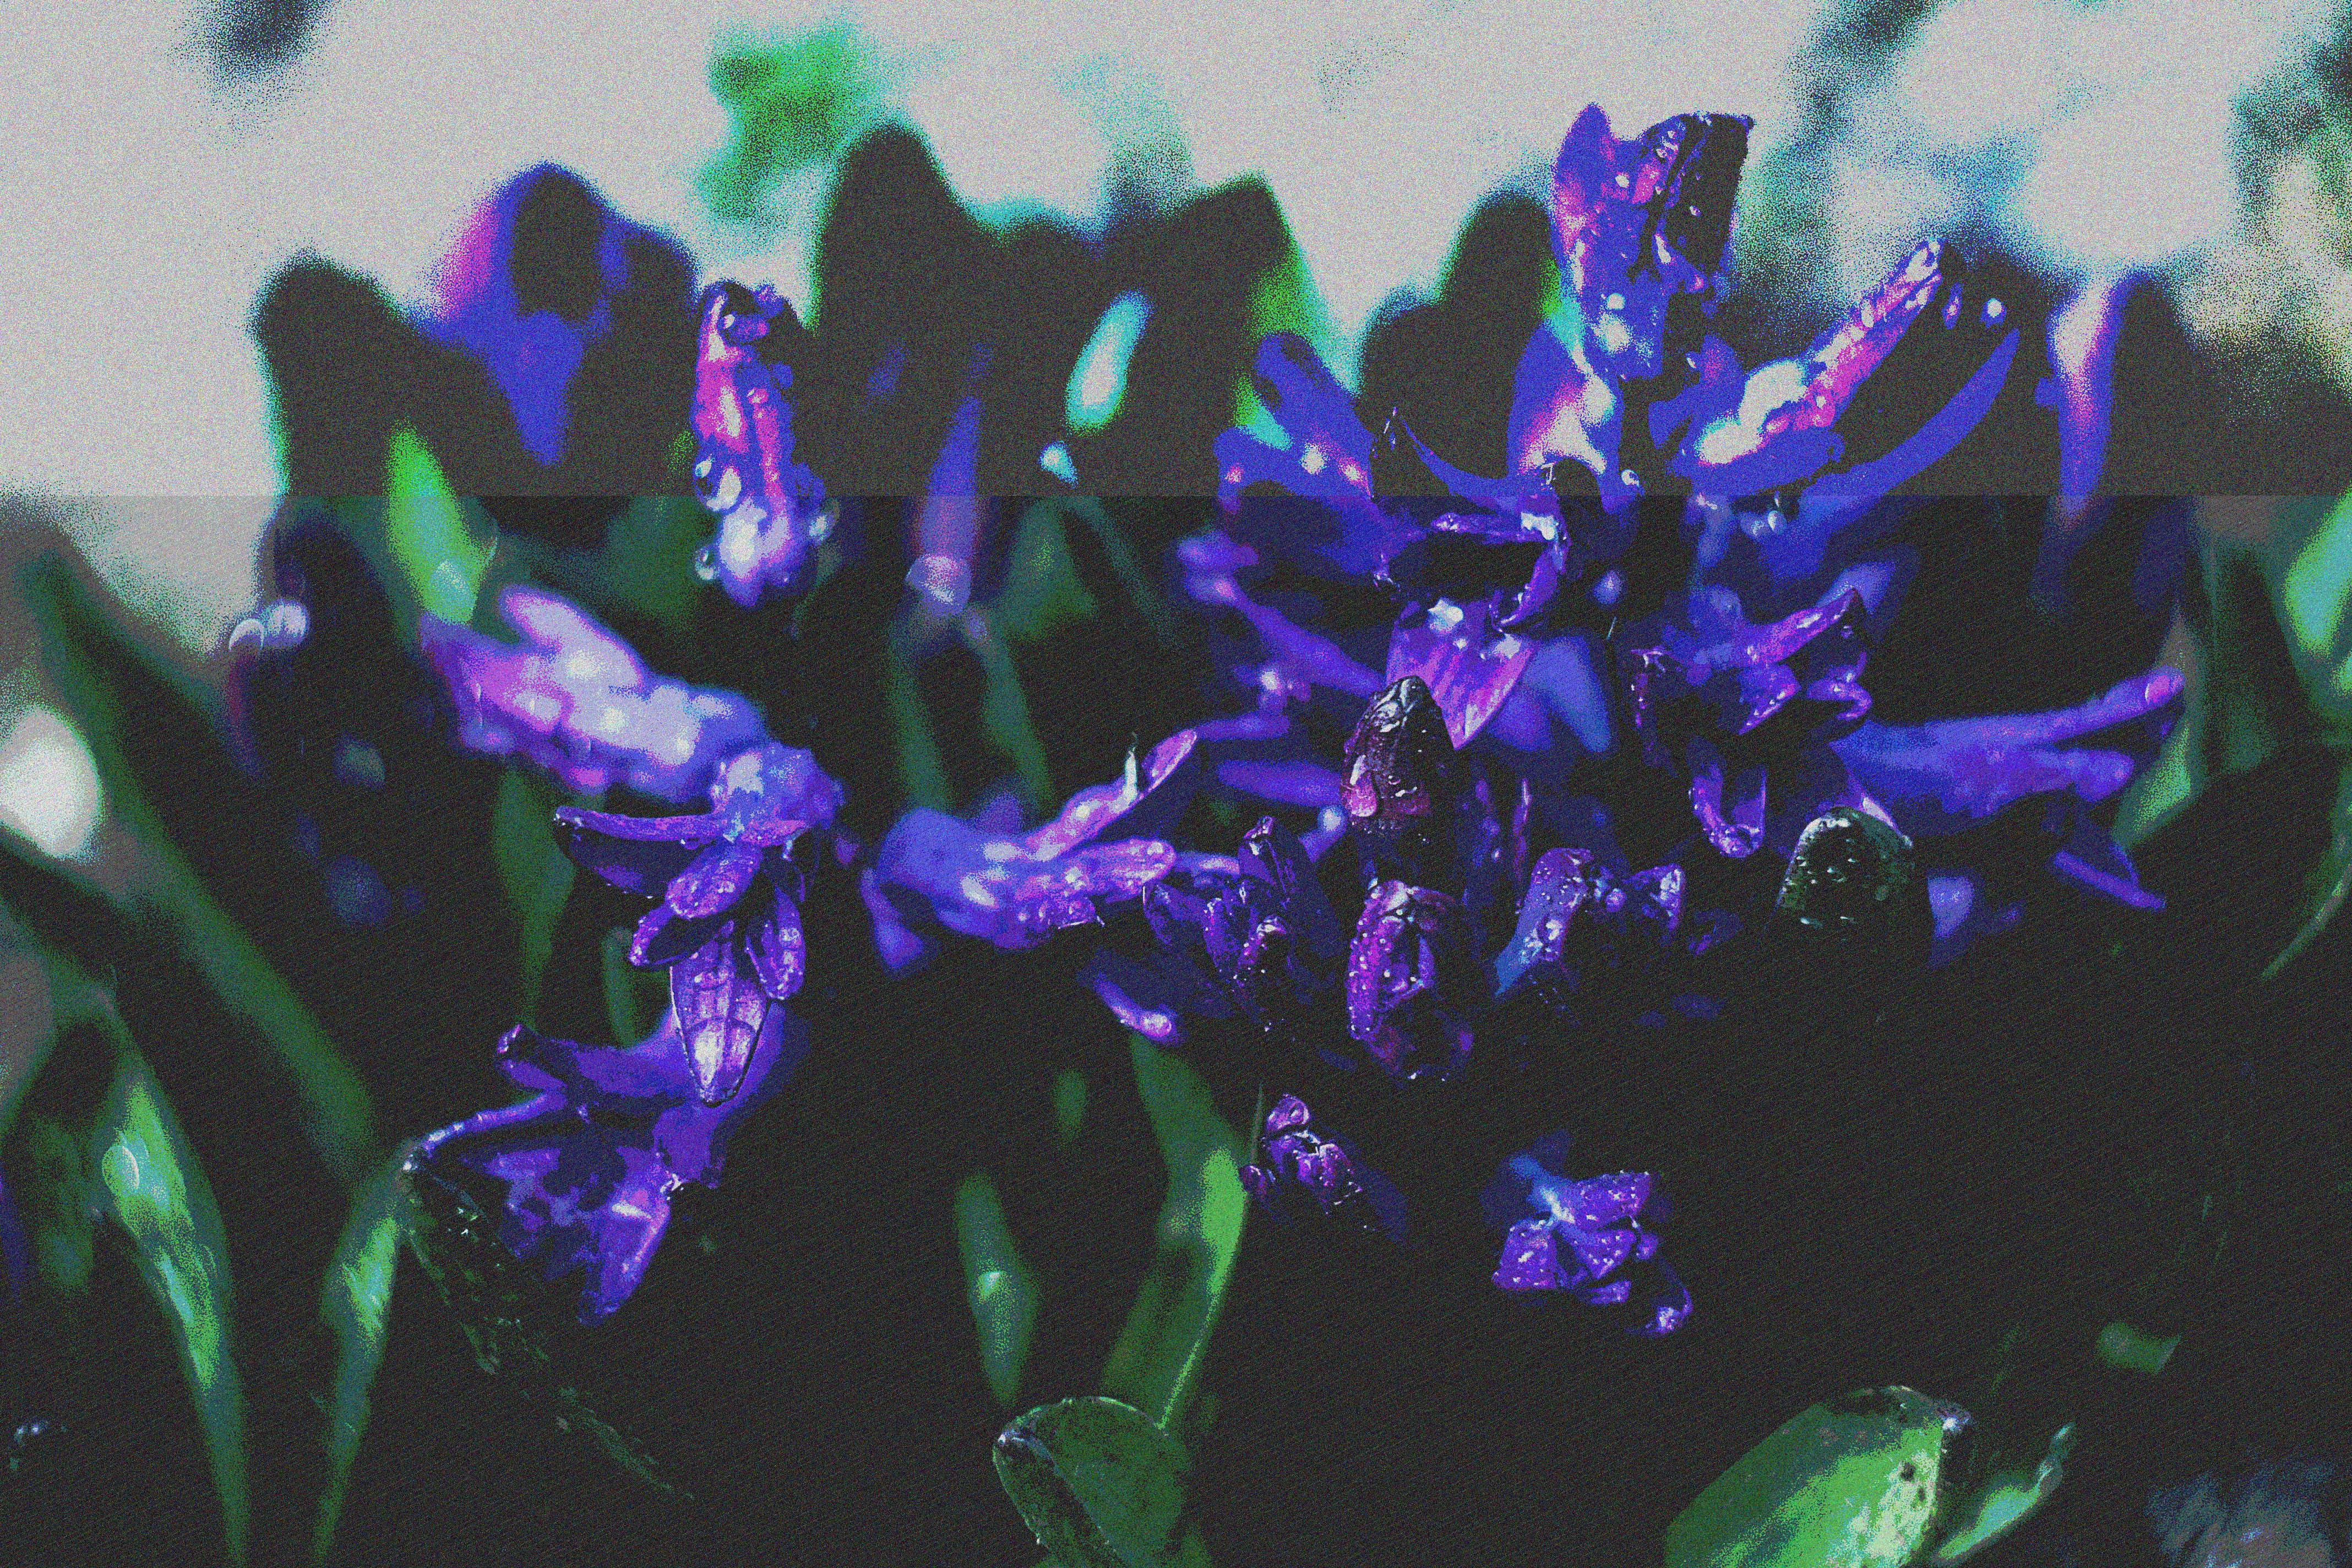
\includegraphics[width=1\textwidth]{flowers-30000000.png}
        \caption*{30 MB Nachricht}
      \end{minipage}
    };

    \matrix [column sep=3.5cm] at ($(original.north)!0.5!(10mb.north) + (0,3.5cm)$) {
      \coordinate (a); & \coordinate (b); & \coordinate (c); & \coordinate (d); \\
    };

    \coordinate (spy-on) at (1.05cm,-0.55cm);

    \spy on ($(original.north) + (spy-on)$) in node[label=below:Original] at (a);
    \spy on ($(10mb.north) + (spy-on)$) in node[label=below:10 MB] at (b);
    \spy on ($(20mb.north) + (spy-on)$) in node[label=below:20 MB] at (c);
    \spy on ($(30mb.north) + (spy-on)$) in node[label=below:30 MB] at (d);


  \end{tikzpicture}
  \caption{Blumen. Größe 4272 $\times$ 2848 Pixel. Maximale Kapazität $\approx 36,5$ MB.
    Gute Bildqualität bis zu 20MB versteckter Nachricht.}
  \label{fig:example-flowers}
\end{figure}
